\subsection{Summarizing Data on Random Variables}

\textbf{Frequency Histogram}
\begin{itemize}
    \item Symmetric: mean = median
    \item Right-skewed: mean > median
    \item Left-skewed: mean < median
\end{itemize}
\begin{definition}[\textbf{Sample}]
    A set of observed outcomes $x_1, \ldots, x_n$ for a random variable $X$
    is a \textbf{sample}.
\end{definition}

\begin{definition}[\textbf{Arithmetic Mean or Sample Mean}]
    The \textbf{mean} of $n$ outcomes $x_1, \ldots, x_n$ for a randome variable
    $X$ is \[\bar{x} = \dis \sum_{i=1}^n \frac{x_i}{n}.\]
\end{definition}

\begin{definition}[\textbf{Median}]
    The \textbf{median} of a sample is a value \st half the results are below it and
    half above it, when the results are arranged in numerical order.
\end{definition}

\begin{note}
    If there are even number of values. The median is the mean of the two middle values.
\end{note}

\begin{definition}[\textbf{Mode}]
    The \textbf{mode} of the sample is the value which occurs most often. 
\end{definition}

\begin{note}
    There can be multiple modes.
\end{note}


\subsection{Expectation of a Random Variable}

\begin{definition}[\textbf{Expected Value (Expectation)}]
    Let $X$ be a discrete random variable with $\operatorname{range}{(X)} = A$ and
    probability function $f(x)$. The \textbf{expected value} of $X$ is given by
    \[\mu = \expect{X} = \sum_{x \in A} xf(x).\]   
\end{definition}

\begin{theorem}[\textbf{Expected Value of $g(X)$}]
    \phantom{}  \\
    Let $X$ be a discrete random variable with $\operatorname{range}{(X)} = A$ and
    probability function $f(x)$. The \textbf{expected value} of some function $g(X)$
    of $X$ is given by
    \[\expect{g(X)} = \sum_{x \in A} g(x)f(x).\]    
\end{theorem}


\begin{note}
    \phantom{}\
    \begin{enumerate}
        \item Interpret $\expect{g(X)}$ as the average value of $g(X)$ in an infinite series of repetitions of the process where $X$ is defined.
        \item $\expect{g(X)}$ may be a value that $g(X)$ never takes.
        \item $\expect{X}$ is NOT a random variable like $X$ but a non-random constant.
        \item Suppose $X$ takes values from 1 to 10. Then $\expect{X}$ cannot exceed 10 or smaller than 1.
    \end{enumerate}
\end{note}

\begin{theorem}[\textbf{Linearity Properties of Expectation}]
    \phantom{}  \
    \begin{enumerate}
        \item For constants $a$ and $b$, \[\dis \expect{ag(X) + b} = a\expect{g(X)} + b.\]
        \item For constants $a$, $b$ and two functions $g_1$, $g_2$, 
        \[\expect{ag_1(X) + bg_2(X)} = a\expect{g_1(X)} + b\expect{g_2(X)}.\]
    \end{enumerate}
\end{theorem}

\begin{note}
    For constant $a$, we have $\expect{a} = a$.
\end{note}

\pagebreak 

\begin{example}
    Suppose we have the random variable $X$ \st $f_X(x) = \frac{x}{10}$, $x = 1,2,3,4$. Find $\expect{X(5-X)}$.

    \textbf{Solution:} \\
    $\expect{X(5-X)} = \expect{5X - X^2} = 5\expect{X} - \expect{X^2} = 5 \left[ (1 \times \frac{1}{10}) + \cdots + (4 \times \frac{4}{10}) \right] - \left[ (1^2 \times \frac{1}{10}) + \cdots + (4^2 \times \frac{4}{10}) \right] \\ = 5 \times 3 - 10 = 5$.
\end{example}


\subsection{Some Applications of Expectation}

\begin{example}
    A local television station sells 15sec, 30sec, and 60sec advertising spots. Let $X$ denote the length of a randomly selected commercial appearing on this
    station, and suppose that the probability distribution of $X$ is given by
    \begin{center}
        \begin{tabular}{l|*{3}{c}}
            $x$ & 15 & 30 & 60 \\
            \hline
            $f(x)$ & $0.1$ & $0.3$ & $0.6$ \\
        \end{tabular}
    \end{center}

    \begin{enumerate}[label=(\alph*)]
        \item Find $\expect{X}$. \\
        \textbf{Solution:} $\expect{X} = \displaystyle \sum_{\text{all $x$}} xf(x) = (15 \times 0.1) + (30 \times 0.3) + (60 \times 0.6) = 46.5$ seconds.
        \item If a 15s spot sells for \$500, a 30s spot for \$800, and a 60s spot for \$1000, find the average amount paid for commercials appearing on this station. \\
        \textbf{Solution:} $\expect{Y} = (500 \times 0.1) + (800 \times 0.3) + (1000 \times 0.6) = \$890$. \\
    \end{enumerate}
    
\end{example}

\subsection{Means and Variances of Distributions}

\begin{definition}[\textbf{Expectation for Probability Models}]
    \phantom{}\
    \begin{enumerate}
        \item Binomial: $\expect{X} = np$.
        \item Poisson: $\expect{X} = \lambda t = \mu$.
        \item Discrete Uniform: $\expect{X} = \dis \frac{a+b}{2}$.
        \item Hypergeometric: $\expect{X} = \dis \frac{nr}{N}$.
        \item Negative Binomial: $\expect{X} = \dis \frac{k(1-p)}{p}$.
        \item Geometric: $\expect{X} = \dis \frac{1-p}{p}$.
    \end{enumerate}
\end{definition}

\begin{definition}[\textbf{Variance}]
    The \textbf{variance} of a random variable $X$, denoted by $\Var{X}$ or $\sigma^2$, is
    \[\sigma^2 = \Var{X} = \expect{(X - \mu)^2}.\]
\end{definition}

\begin{note}
    Variance is the average square of the distance from the mean ($\text{units}^2$).
\end{note}

The definition of variance is not efficient to use for calculation of $\Var{X}$, whereas
the following two results are often useful:
\begin{theorem}
    \phantom{}\
    \begin{enumerate}
        \item $\dis \Var{X} = \expect{X^2} - \left[\expect{X}\right]^2 = \expect{X^2} - \mu^2$
        \item $\dis \Var{X} = \expect{X(X - 1)} + \expect{X} - \left[\expect{X}\right]^2 = \expect{X(X - 1)} + \mu - \mu^2$
    \end{enumerate}
\end{theorem}

\begin{definition}[\textbf{Standard Deviation}]
    The \textbf{standard deviation} of a random variable $X$ is
    \[\sigma = \operatorname{sd}{(X)} = \sqrt{\Var{X}} = \sqrt{\expect{(X - \mu)^2}}\]
\end{definition}

\begin{figure}[htbp]
    \center
    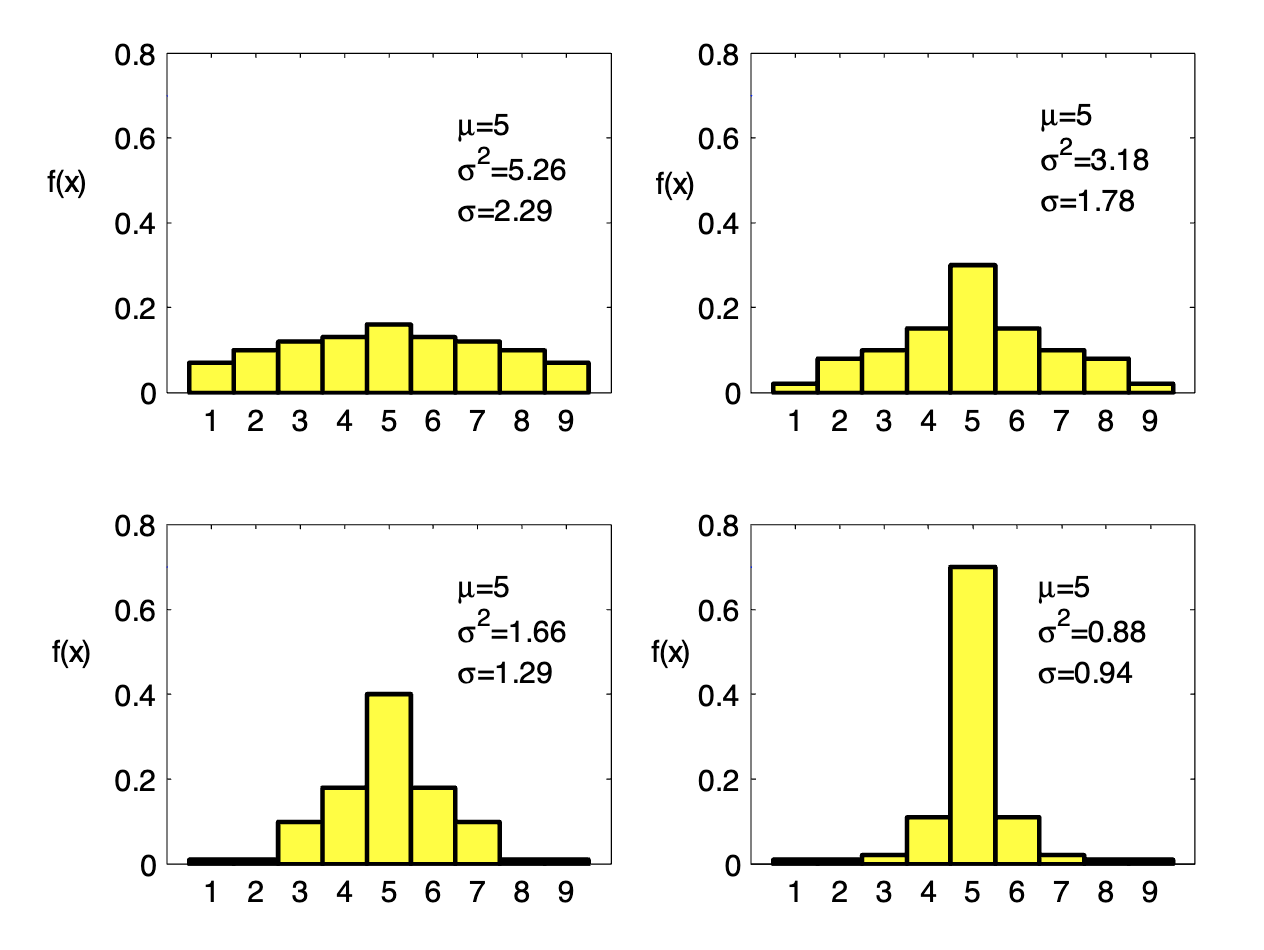
\includegraphics[scale=0.55]{img/var-and-sd.png}
    \caption{How $\Var{X}$ or $\operatorname{sd}(X)$ reflects the spread of a probability histogram.}
\end{figure}

\begin{definition}[\textbf{Variance for Probability Models}]
    \phantom{}\
    \begin{enumerate}
        \item Binomial: $\Var{X} = np(1-p)$.
        \item Poisson: $\Var{X} = \mu$.
        \item Discrete Uniform: $\Var{X} = \dis \frac{(b-a+1)^2 - 1}{12}$.
        \item Hypergeometric: $\Var{X} = \dis \frac{nr}{N} \left( 1 - \frac{r}{N} \right) \frac{N-n}{N-1}$.
        \item Negative Binomial: $\Var{X} = \dis \frac{k(1-p)}{p^2}$.
        \item Geometric: $\Var{X} = \dis \frac{1-p}{p^2}$.
    \end{enumerate}
\end{definition}

\begin{theorem}[\textbf{Properties of Mean and Variance}]
    \phantom{}  \\
    If $a$ and $b$ are constants and $Y = aX + b$, then
    \[\mu_Y = \expect{Y} = a\expect{X} + b = a\mu_X + b\] and
    \[\sigma_Y^2 = \Var{Y} = a^2\Var{X} = a^2\sigma_X^2,\]
    where $\mu_X = \expect{X}$, $\sigma_X^2 = \Var{X}$, $\expect{Y} = \mu_Y$, and $\Var{Y} = \sigma_Y^2.$
\end{theorem}

\begin{note}
    For constant $a$, we have $\Var{a} = 0$.
\end{note}




\newpage